\documentclass{article}
\usepackage{indentfirst}
\usepackage{multirow}\usepackage{makecell}\usepackage{diagbox}
\setlength{\parindent}{2em}
\usepackage{xeCJK}\usepackage{float}
\usepackage{xcolor}\usepackage{tcolorbox}
\usepackage{colortbl}
\usepackage{graphicx}
\usepackage{subfig}
\setCJKmainfont{SimSun} 
\usepackage{tikz}            % 添加 TikZ 包以支持 tikzpicture 环境
\usepackage{pgfplots}        % 核心绘图包
\usepgfplotslibrary{patchplots}
\pgfplotsset{compat=1.17}
\usepackage{amsmath}
\usepackage{amssymb}
\usepackage{amsthm}
\usepackage{geometry}
\usepackage{tocbibind}
\usepackage{hyperref}
\usepackage{enumitem}
\geometry{a4paper,margin=2.5cm}


\title{ 导数复习学案(天津专用)}
\author{小白高考数学}
\date{}

\hypersetup{
    colorlinks=true,    % 链接文字上色（false则加边框）
    linkcolor=black,     % 目录跳转链接颜色（黑色）
    urlcolor=blue,      % 网址链接颜色
    citecolor=green,    % 引用链接颜色
    bookmarks=true,     % 生成PDF书签（侧边栏）
    bookmarksnumbered=true, % 书签显示章节号
    pdfstartview=FitH   % PDF打开时自适应宽度
}

\renewcommand{\contentsname}{目录}
\begin{document}
\maketitle

\vspace{30\baselineskip}
\begin{center}
迟序之数，非出神怪，有形可检，有数可推
\end{center}
\begin{flushright}
    \rightskip=7em 
——祖冲之《缀术》
\end{flushright}    
\newpage
\tableofcontents % 核心命令：生成目录
\newpage 

\section{知识要点}
\subsection{导数的概念与意义}
\subsubsection{导数的概念}

\begin{figure}[h]
    \centering
    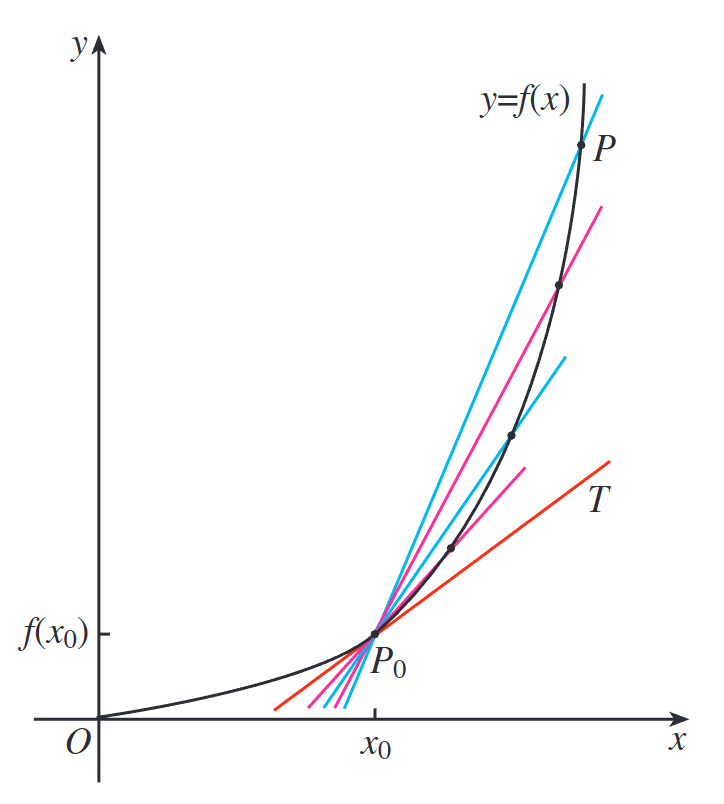
\includegraphics[width=0.5\textwidth]{切线.png}
\end{figure}

一个函数在一点的导数代表着这个函数在该点的瞬时变化率。
\subsubsection{导数的意义}

$\diamond $ 物理意义：

很多物理量均由导数定义，例如：速度是位移对时间的导数，表示物体位置随时间的变化率；加速度是速度对时间的导数，表示物体速度随时间的变化率；电流是电荷量对时间的导数，表示电荷量随时间的变化率；功率是能量对时间的导数，表示能量随时间的变化率。

$\diamond $ 几何意义：

导数的几何意义是函数图像在某一点处切线的斜率，即：
\[
\text{即 } k_0 = \lim_{\Delta x \to 0} \frac{f(x_0 + \Delta x) - f(x_0)}{\Delta x} = f'(x_0).
\]

这些导数连缀成的新函数便成为导函数：当 \(x = x_0\) 时，\(f'(x_0)\) 是一个唯一确定的数。这样，当 \(x\) 变化时，\(y = f'(x)\) 就是 \(x\) 的函数，我们称它为 \(y = f(x)\) 的导函数（简称导数）。\(y = f(x)\) 的导函数有时也记作 \(y'\)，即
\[
f'(x) = y' = \lim_{\Delta x \to 0} \frac{f(x + \Delta x) - f(x)}{\Delta x}.
\]

导函数的正负性反映了原函数的单调性，导函数的值则具体描绘了原函数增减的幅度.同样的，导数的导数（即二阶导数）则反映了一阶导数的变化情况，进而更加细致的描绘了原函数的增减变化。例如：若一个函数在某一区间内一二阶导数均大于0，说明这个函数在该区间单调递增并且增速不断加快。
\newpage
例一\;\;已知函数 \(y = f(x)\) 的图象是下列四个图象之一，且其导函数 \(y = f'(x)\) 的图象如图所示，则该函数的图象是（\quad ）

\begin{figure}[H]
    \centering
    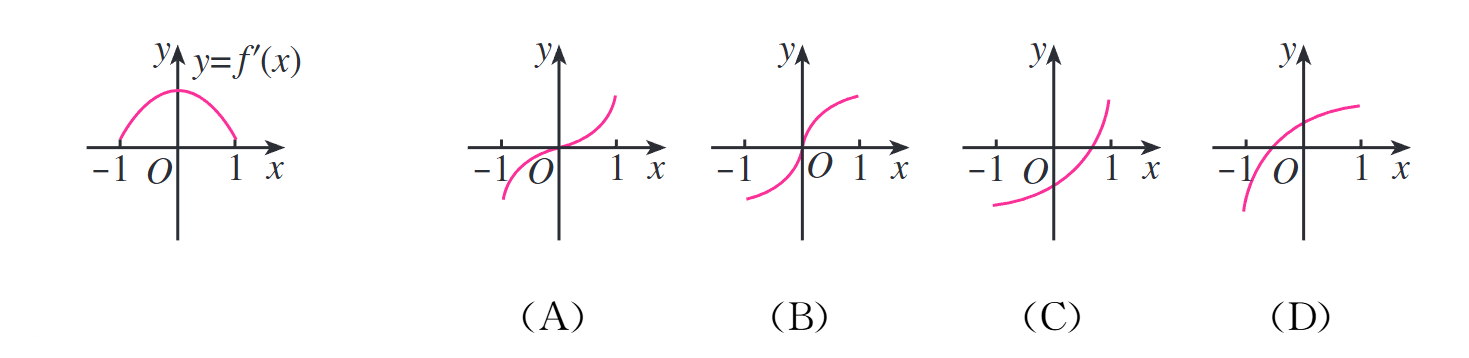
\includegraphics[width=1.0\textwidth]{image4.png}
\end{figure}


例二\;\;如图，直线 \(l\) 和圆 \(P\)，当 \(l\) 从 \(l_0\) 开始在平面上按逆时针方向绕点 \(O\) 匀速转动（转动角度不超过 \(90^\circ\)）时，它扫过的圆内阴影部分的面积 \(S\) 是时间 \(t\) 的函数。这个函数的图象大致是（\quad ）。

\begin{figure}[h]
    \centering
    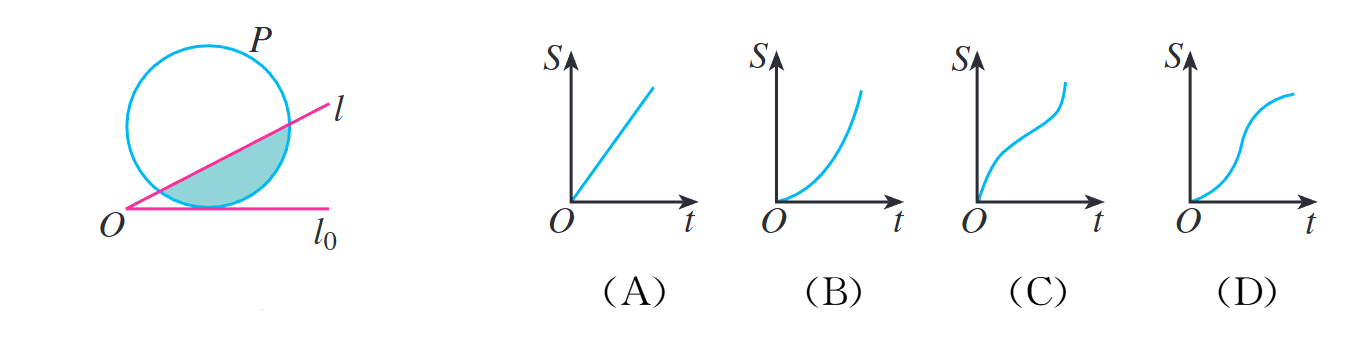
\includegraphics[width=1.0\textwidth]{image5.png}
\end{figure}

\begin{center}

    \vspace{5\baselineskip}
\textbf{微专题：切线问题}
\end{center}
\;\;切线问题大致分为：

$\blacklozenge $ 求函数图像上某点的切线（已知切点，切线唯一）；

$\blacklozenge $ 求曲线过函数图像外一点的切线（未知切点设切点），值得注意的是，对于一些函数而言，满足要求的切线未必唯一；

$\blacklozenge $ 涉及多个函数，多条切线的综合问题
\vspace{2\baselineskip}

例一 \;\;求下列曲线在给定点处的切线方程：
\begin{enumerate}
    \item \(y = x - \dfrac{1}{x}\)，\((1,\ 0)\);
    \item \(y = \dfrac{\mathrm{e}^{2x - 1}}{x^2}\)，\(\left(\dfrac{1}{2},\ 4\right)\).
\end{enumerate}
\newpage

例二 \;\; 已知曲线 \(f(x) = x^3 + 1\)。
\begin{enumerate}
    \item 求过点 \(M(1,1)\) 的曲线 \(f(x)\) 的切线方程；
    \item 求过点 \(N(2,9)\) 的曲线 \(f(x)\) 的切线方程。
\end{enumerate}

\vspace{20\baselineskip}

例三 \;\;已知曲线 \(y = x + \ln x\) 在点 \((1, 1)\) 处的切线与曲线 \(y = ax^2 + (2a + 3)x + 1\) 只有一个公共点，求 \(a\) 的值

\vspace{15\baselineskip}

例四\;\; 已知函数 \(f(x) = \mathrm{e}^x\)，\(g(x) = \ln x\)，证明：存在直线 \(l\)，使 \(l\) 既是曲线 \(y = f(x)\) 的切线，也是曲线 \(y = g(x)\) 的切线
\newpage

\subsection{导数的运算}
\subsubsection{初等函数的导数}
\begin{table}[htbp]
  \centering
  \begin{tabular}{|p{0.95\textwidth}|}
    \hline
    \rowcolor{blue!20}
    \multicolumn{1}{|c|}{\large 基本初等函数的导数公式} \\
    \hline
    1. 若 \(f(x)=c\)（\(c\) 为常数），则 \(f'(x)=0\); \\[4pt]
    2. 若 \(f(x)=x^\alpha\)（\(\alpha\in\mathbb{R}\)，且 \(\alpha\neq0\)），则 \(f'(x)=\alpha x^{\alpha-1}\); \\[4pt]
    3. 若 \(f(x)=\sin x\)，则 \(f'(x)=\cos x\); \\[4pt]
    4. 若 \(f(x)=\cos x\)，则 \(f'(x)=-\sin x\); \\[4pt]
    5. 若 \(f(x)=a^x\)（\(a>0\)，且 \(a\neq1\)），则 \(f'(x)=a^x\ln a\); \\[4pt]
    \quad 特别地，若 \(f(x)=e^x\)，则 \(f'(x)=e^x\); \\[4pt]
    6. 若 \(f(x)=\log_a x\)（\(a>0\)，且 \(a\neq1\)），则 \(f'(x)=\dfrac{1}{x\ln a}\); \\[8pt]
    \quad 特别地，若 \(f(x)=\ln x\)，则 \(f'(x)=\dfrac{1}{x}.\) \\[4pt]
    \hline
  \end{tabular}
\end{table}
\subsubsection{导数的四则运算}
\begin{enumerate}
    \item \textbf{和差法则}：两个函数和（差）的导数，等于这两个函数导数的和（差）
    \[
    [u(x) \pm v(x)]' = u'(x) \pm v'(x)
    \]

    \item \textbf{乘法法则}：两个函数积的导数，等于第一个函数的导数乘第二个函数，加上第一个函数乘第二个函数的导数
    \[
    [u(x) \cdot v(x)]' = u'(x)v(x) + u(x)v'(x)
    \]
    特别地，若 \(c\) 为常数，则 \( [c \cdot u(x)]' = c \cdot u'(x) \)

    \item \textbf{除法法则}：两个函数商的导数，等于分子的导数乘分母，减去分子乘分母的导数，再除以分母的平方（\(v(x) \neq 0\)）
    \[
    \left[\frac{u(x)}{v(x)}\right]' = \frac{u'(x)v(x) - u(x)v'(x)}{[v(x)]^2}
    \]
\end{enumerate}

\noindent \textbf{例一} \;\;求下列函数的导数：

\begin{enumerate}
    \item \(y = x^3 e^x\);
    \item \(y = \dfrac{2\sin x}{x^2}\);
    \item \(y = \dfrac{e^x}{\ln x}\).
\end{enumerate}
\subsubsection{复合函数的导数}

一般地，对于由函数 \(y = f(u)\) 和 \(u = g(x)\) 复合而成的函数 \(y = f(g(x))\)，它的导数与函数 \(y = f(u)\)，\(u = g(x)\) 的导数间的关系为
\[
\boxed{y_x' = y_u' \cdot u_x'.}
\]

\noindent \textbf{例一} \;\;求下列函数的导数：

\begin{enumerate}
    \item \(y = (3x + 5)^3\);
    \item \(y = e^{-0.05x + 1}\);
    \item \(y = \ln(2x - 1)\);
    \item \(y = \sin(4x^2 + 1)\);
    \item \(y = x^x\).  \fbox{
  tips:利用对数的性质$b=a^{log_a b}$将其转化为复合函数
}
\end{enumerate}



\subsection{利用导数研究函数}

\subsubsection{函数的单调性}
在某个区间 \((a, b)\) 内，函数单调性与导数的关系如下：

\begin{enumerate}
    \item 如果 \(f'(x) > 0\)，那么函数 \(y = f(x)\) 在区间 \((a, b)\) 内单调递增；
    \item 如果 \(f'(x) < 0\)，那么函数 \(y = f(x)\) 在区间 \((a, b)\) 内单调递减。
\end{enumerate}

\vspace{1\baselineskip}
\noindent \textbf{例一} \;\;利用导数判断下列函数的单调性：

\begin{enumerate}
    \item \(f(x) = \frac{1}{3}x^3-\frac{1}{2}x^2 -2x+1\);
    \item \(f(x) = \sin x - x\)，\(x \in (0, \pi)\);
    \item \(f(x)=\cos(x)-\frac{1}{2}x^2+1\)
\end{enumerate}
\vspace{6\baselineskip}
\fbox{
  \parbox{0.95\textwidth}{
    判断函数 \(y = f(x)\) 单调性的核心步骤如下：
    \begin{enumerate}
        \item \textbf{第1步：确定函数的定义域} \\
        注：单调区间是定义域的子集，需先明确函数的有效取值范围，再讨论单调性。
        
        \item \textbf{第2步：求出导数 \(f'(x)\) 的零点} \\
        导数的零点是划分函数单调区间的关键分界点。
        
        \item \textbf{第3步：划分区间并判断导数符号} \\
        用 \(f'(x)\) 的零点将 \(f(x)\) 的定义域划分为若干个区间，列表给出 \(f'(x)\) 在每个区间上的正负性，根据导数符号确定函数单调性。
    \end{enumerate}
  }
}
\vspace{2\baselineskip}

\noindent \textbf{例二}（江苏高考节选）已知函数 \(f(x) = x^3 + ax^2 + b\)（\(a,b \in \mathbb{R}\)），试讨论 \(f(x)\) 的单调性。
\vspace{15\baselineskip}

\fbox{
  \parbox{0.95\textwidth}{
    tips：如果函数$f(x)$满足：$f'(x)>(<)0,\forall x\in (a,b)\bigcup (c,d)$,其中$a<b<c<d$,
    则函数$f(x)$在区间$(a,b)$和$(c,d)$内单调递增(递减)，或者说$(a,b)$和$(c,d)$都是$f(x)$的单调递增（递减）区间。但不能说函数在$(a,d)\bigcup (c,d)$上单调递增（递减）。
    $f(x)=\frac{1}{x}$就是一个很好的例子。它在$(-\infty,0)$和$(0,+\infty)$内单调递减，但不能说它在$(-\infty,+\infty)$上单调递减。
    读者可以利用函数单调性的定义证明之。        
   
  }
}

\vspace{4\baselineskip}

\noindent \textbf{例三} \;\;设函数 \(f(x) = ax - \dfrac{1}{x} - \ln x\)（\(a \in \mathbb{R}\)），讨论函数 \(f(x)\) 的单调性
\vspace{30\baselineskip}

\noindent \textbf{例四}（2021新高考二卷节选）已知函数 \(f(x) = (x - 1)\mathrm{e}^x - ax^2 + b\)。讨论 \(f(x)\) 的单调性

\newpage
\begin{center}
\subsubsection*{微专题：构造函数解不等式}
\end{center}

\noindent \textbf{经典例题}:\;\;函数 \(f(x)\) 是定义在 \(\mathbb{R}\) 上的奇函数，且对任意的 \(x \in \mathbb{R}\)，\(f(x) + f'(x) > 1\)，则不等式 \(\mathrm{e}^x f(x) > \mathrm{e}^x - 1\) 的解集是(\;\;\;)

\begin{enumerate}
    \item[A.] \(\{x \mid x > 0\}\)
    \item[B.] \(\{x \mid x < 0\}\)
    \item[C.] \(\{x \mid x < -1 \text{ 或 } x > 1\}\)
    \item[D.] \(\{x \mid x < -1 \text{ 或 } 0 < x < 1\}\)
\end{enumerate}

\noindent \textbf{解析}
\begin{enumerate}
    \item[\textbf{第一步:}] \textbf{构造目标函数.} \\
    设 \(g(x) = \mathrm{e}^x [f(x) - 1]\).

    \item[\textbf{第二步:}] \textbf{求目标函数的导数.} \\
    则 \(g'(x) = \mathrm{e}^x [f(x) + f'(x) - 1]\).

    \item[\textbf{第三步:}] \textbf{确定导数的符号并指出目标函数的单调性.} \\
    因为 \(f(x) + f'(x) > 1\), 所以 \(g'(x) > 0\), 即 \(g(x)\) 在 \(\mathbb{R}\) 上单调递增.

    \item[\textbf{第四步:}] \textbf{确定目标函数的特殊函数值.} \\
    又 \(f(x)\) 是定义在 \(\mathbb{R}\) 上的奇函数, 所以 \(f(0) = 0\), 则 \(g(0) = -1\).

    \item[\textbf{第五步:}] \textbf{由目标函数单调性得出结论.} \\
    不等式 \(\mathrm{e}^x f(x) > \mathrm{e}^x - 1\), 即 \(g(x) > g(0)\), 由 \(g(x)\) 的单调性得 \(x > 0\).
\end{enumerate}

\newpage
\begin{tcolorbox}[
    colback=white,
    colframe=black,
    boxrule=0.8pt,
    left=10pt,
    right=10pt,
    top=10pt,
    bottom=10pt
]
这类题目的本质是研究与导数相关的四则运算的结构及函数的单调性，因此熟悉结构，准确构造函数是关键。构造函数有以下几种方法。

\begin{enumerate}
    \item 对于 \(f'(x) > g'(x)\)，可构造函数 \(h(x) = f(x) - g(x)\)。更一般地，若 \(f'(x) > k\)（\(k \neq 0\)），即导数大于某个非零常数，则可构造函数 \(g(x) = f(x) - kx + b\)。

    \item 对于 \(f'(x) + g'(x) > 0\)，可构造函数 \(h(x) = f(x) + g(x)\)。

    \item 对于 \(f'(x)g(x) + f(x)g'(x) > 0\)，可构造函数 \(h(x) = f(x)g(x)\)。

    特别地，
    \begin{enumerate}
        \item 对于 \(f'(x) + f(x) > 0\)，可构造函数 \(h(x) = e^x f(x)\)；
        \item 对于 \(xf'(x) + f(x) > 0\)，可构造函数 \(h(x) = xf(x)\)；
        \item 对于不等式 \(f'(x) + kf(x) > 0\)，可构造函数 \(h(x) = e^{kx}f(x)\)；
        \item 对于不等式 \(f'(x) + \ln a \cdot f(x) > 0\)，可构造函数 \(h(x) = a^x f(x)\)；
        \item 对于不等式 \(xf'(x) + nf(x) > 0\)，可构造函数 \(h(x) = x^n f(x)\)；
        \item 对于不等式 \(f'(x) + 2xf(x) > 0\)，可构造函数 \(h(x) = e^{x^2}f(x)\)；
        \item 对于不等式 \(f'(x)\ln x + \dfrac{f(x)}{x} > 0\)，可构造函数 \(h(x) = f(x)\ln x\)。
    \end{enumerate}

    \item 对于 \(f'(x)g(x) - f(x)g'(x) > 0\)，可构造函数 \(h(x) = \dfrac{f(x)}{g(x)}\)。

    特别地，
    \begin{enumerate}
        \item 对于 \(f'(x) > f(x)\)（或 \(f'(x) - f(x) > 0\)），可构造函数 \(h(x) = \dfrac{f(x)}{e^x}\)；
        \item 对于 \(xf'(x) - f(x) > 0\)，可构造函数 \(h(x) = \dfrac{f(x)}{x}\)（\(x \neq 0\)）；
        \item 对于不等式 \(xf'(x) - nf(x) > 0\)，可构造函数 \(h(x) = \dfrac{f(x)}{x^n}\)（\(x \neq 0\)）。
    \end{enumerate}
\end{enumerate}
\end{tcolorbox}

\noindent 例一 （2024·湖南省张家界市慈利一中期中）已知函数 \(f(x) - f'(x) > 0\)，\(f(0) = 1\)，则关于 \(x\) 的不等式 \(f(x) > \mathrm{e}^x\) 的解集为(\;\;\;)

\begin{enumerate}
    \item[A.] \(\{x \mid x > 0\}\)
    \item[B.] \(\{x \mid x < 0\}\)
    \item[C.] \(\{x \mid x < 1\}\)
    \item[D.] \(\{x \mid x > 1\}\)
\end{enumerate}

\newpage

\subsubsection{极值与最值}

$\diamond$ 极值：

\begin{table}[H]
  \centering
  \begin{tabular}{|c|c|c|}
    \hline
    & \textbf{极小值} & \textbf{极大值} \\
    \hline
    \textbf{定义} & 
    \parbox{0.4\textwidth}{
      若函数 \(y = f(x)\) 在点 \(x = a\) 的函数值 \(f(a)\) 比它在点 \(x = a\) 附近其他点的函数值都小，\(f'(a) = 0\)；而且在点 \(x = a\) 附近的左侧 \(f'(x) < 0\)，右侧 \(f'(x) > 0\)，其实就是\(f''(x)>0\).就把 \(a\) 叫做函数 \(y = f(x)\) 的极小值点，\(f(a)\) 叫做函数 \(y = f(x)\) 的极小值。
    }
    & 
    \parbox{0.4\textwidth}{
      若函数 \(y = f(x)\) 在点 \(x = b\) 的函数值 \(f(b)\) 比它在点 \(x = b\) 附近其他点的函数值都大，\(f'(b) = 0\)；而且在点 \(x = b\) 附近的左侧 \(f'(x) > 0\)，右侧 \(f'(x) < 0\)，其实就是\(f''(x)<0\).就把 \(b\) 叫做函数 \(y = f(x)\) 的极大值点，\(f(b)\) 叫做函数 \(y = f(x)\) 的极大值。
    } \\
    \hline
    \textbf{图象} & 
    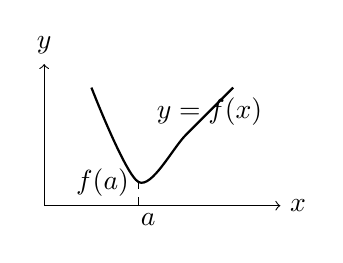
\begin{tikzpicture}[scale=0.6]
      \draw[->] (0,0) -- (5,0) node[right] {$x$};
      \draw[->] (0,0) -- (0,3) node[above] {$y$};
      \draw[thick] plot[smooth] coordinates {(1,2.5) (2,0.5) (3,1.5) (4,2.5)};
      \draw[dashed] (2,0) -- (2,0.5) node[left] {$f(a)$};
      \node at (2.2, -0.3) {$a$};
      \node at (3.5, 2) {$y=f(x)$};
    \end{tikzpicture}
    & 
    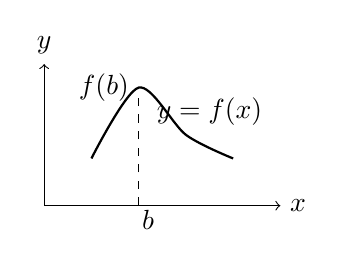
\begin{tikzpicture}[scale=0.6]
      \draw[->] (0,0) -- (5,0) node[right] {$x$};
      \draw[->] (0,0) -- (0,3) node[above] {$y$};
      \draw[thick] plot[smooth] coordinates {(1,1) (2,2.5) (3,1.5) (4,1)};
      \draw[dashed] (2,0) -- (2,2.5) node[left] {$f(b)$};
      \node at (2.2, -0.3) {$b$};
      \node at (3.5, 2) {$y=f(x)$};
    \end{tikzpicture} \\
    \hline
  \end{tabular}
\end{table}
即：
\vspace{2\baselineskip}
\begin{center}
\begin{tabular}{|c|c|c|c|}
\hline
$x$ & $(-\infty,x_0)$ & $x_0$ & $(x_0,+\infty)$ \\
\hline
$f'(x)$ & $+$ & $0$ & $-$ \\
\hline
$f(x)$ & 单调递增$\nearrow$ & 极大值$f(x_0)$ & 单调递减$\searrow$ \\
\hline
\end{tabular}
\end{center}

\vspace{1em} % 两个表格之间增加1em间距，避免拥挤

% 表格2：极小值判断表
\begin{center}
\begin{tabular}{|c|c|c|c|}
\hline
$x$ & $(-\infty,x_0)$ & $x_0$ & $(x_0,+\infty)$ \\
\hline
$f'(x)$ & $-$ & $0$ & $+$ \\
\hline
$f(x)$ & 单调递减$\searrow$ & 极小值$f(x_0)$ & 单调递增$\nearrow$ \\
\hline
\end{tabular}
\end{center}
\vspace{2\baselineskip}

$\diamond$  最值：
\vspace{1\baselineskip}

对于区间$D$上的函数$y=f(x)$,如果存在$x_0\in D$,使得对于任意的$x\in D$,恒有$f(x)\leq f(x_0)$,则称函数$y=f(x)$在区间$D$上取得最大值$f(x_0)$;如果存在$x_0\in D$,使得对于任意的$x\in D$,恒有$f(x)\geq f(x_0)$,则称函数$y=f(x)$在区间$D$上取得最小值$f(x_0)$.

需要注意的是：函数并不必然在一个区间上能去到最大（最小）值，例如函数$y=\frac{1}{x}$在区间$(0,+\infty)$上没有最大值，在区间$(-\infty,0)$上没有最小值。不过，对于一个连续函数$y=f(x)$,如果定义域是一个闭区间$[a,b]$,则函数$y=f(x)$在区间$[a,b]$上必然能去到最大值和最小值。
连续函数指的是一个没有间断点的函数，即这个函数图像是一条连续不断的曲线。

考虑到一个连续函数在闭区间上的最大（最小）值只能从以下两种情况中产生：
1. 函数在区间内的某个点处取得极值（即导数为零，且导函数在该点的两侧变号的点）；
2. 函数在区间的端点处取得值。

因此一个闭区间上的最值问题通常可以通过以下步骤来解决：
1. 首先，确定函数的定义域，并找到函数在该区间内的极值点。
2. 其次，计算函数在这些极致点以及区间的端点处的函数值。
3. 最后，比较这些函数值，确定其中的最大值和最小值。
\vspace{2\baselineskip}

\fbox{
  \parbox{0.95\textwidth}{
    tips：函数的极值是一个局部概念，指的是函数在某个点附近的函数值相对于该点的函数值的大小关系；而函数的最值是一个全局概念，指的是函数在整个定义域内的函数值相对于某个特定点的函数值的大小关系。因此，极值不一定是最值，而最值一定是极值。        
   
  }
}
\vspace{2\baselineskip}
\newpage

\noindent \textbf{例一} \;\;求下列函数的极值：
\begin{enumerate}
    \item \(f(x) = \mathrm{e}^x - x\);
    \item \(f(x) = x - \ln(x + 1)\);
    \item \(f(x) = \dfrac{\ln x}{x}\);
    \item \(f(x) = x^2 \mathrm{e}^{-x}\).
\end{enumerate}
\vspace{10\baselineskip}

\noindent \textbf{例二}\;\;求下列函数的最值：
\begin{enumerate}
    \item  \(f(x) = \dfrac{1}{2}x + \sin x\)，\(x \in [0, 2\pi]\) 
    \item  \(f(x) = \dfrac{x}{\mathrm{e}^{2x}}\)（\(\mathrm{e} = 2.718\ 28\cdots\) 
    \item  \(f(x) = \dfrac{x^2}{1 + x} - \dfrac{3}{4}\ln x\) 
\end{enumerate}
\vspace{10\baselineskip}

\noindent \textbf{例三}\;\;用测量工具测量某物体的长度，由于工具的精度以及测量技术的原因，测量 \(n\) 次得到的数据为：\(a_1, a_2, a_3, \dots, a_n\)。记这 \(n\) 个数据的平均值为 \(\bar{x}\)，即
\[
\bar{x} = \frac{1}{n}\sum_{i=1}^{n} a_i.
\]

证明：当 \(x = \bar{x}\) 时，函数
\[
f(x) = \frac{1}{n}\sum_{i=1}^{n} (a_i - x)^2
\]
取得最小值.
\newpage

\noindent \textbf{例四}（2022全国乙卷）已知函数 \(f(x) = ax - \dfrac{1}{x} - (a + 1)\ln x\)。
\begin{enumerate}
    \item 当 \(a = 0\) 时，求 \(f(x)\) 的最大值；
    \item 若 \(f(x)\) 恰有一个零点，求 \(a\) 的取值范围。
\end{enumerate}
\vspace{30\baselineskip}

\noindent \textbf{例五}（2024广东省阳江市阳春一中月考）若对任意的 \(x \in (0, +\infty)\)，\(ax - \ln(2x) \ge 1\) 恒成立，求实数 \(a\) 的最小值
\newpage

\subsubsection{导函数与原函数的性质关系}
导函数与原函数的性质关系如下：
\begin{enumerate}
    \item 如果函数 \(f(x)\) 是偶函数，那么它的导函数 \(f'(x)\) 是奇函数;如果函数 \(f(x)\) 的定义域包括0，反之就能成立。
    \item 如果函数 \(f(x)\) 是奇函数，那么它的导函数 \(f'(x)\) 是偶函数；反正不成立。
    \item 如果函数 \(f(x)\) 既不是奇函数也不是偶函数，那么它的导函数 \(f'(x)\) 也既不是奇函数也不是偶函数。
    \item 如果函数 \(f(x)\) 是常数函数，那么它的导函数 \(f'(x)\) 是零函数，零函数既是奇函数也是偶函数。
    \item 如果函数 \(f(x)\) 是周期函数，那么它的导函数 \(f'(x)\) 也是周期函数。
    \item 如果函数 \(f(x)\) 是单调函数，那么它的导函数 \(f'(x)\) 的符号在相应的单调区间内保持不变。
\end{enumerate}

1.的简要证明：

已知 \(g(x) = f'(x)\) 是奇函数，即 \(g(-x) = -g(x)\)。
构造函数 \(h(x) = f(x) - f(-x)\)，求导得：
\[
h'(x) = f'(x) + f'(-x) = g(x) + g(-x) = g(x) - g(x) = 0
\]
因此 \(h(x)\) 是常数函数，即 \(h(x) = C\)，其中 \(C\) 为常数。
\[
f(x) - f(-x) = C
\]

若 \(f(x)\) 的定义域包含 \(0\)，令 \(x = 0\)，则 \(C = f(0) - f(0) = 0\)。
此时 \(f(x) - f(-x) = 0\)，即 \(f(x) = f(-x)\)，故 \(f(x)\) 是偶函数。
\vspace{2\baselineskip}

\noindent \textbf{【经典例题】} （2022新高考一卷）已知函数 \(f(x)\) 及其导函数 \(f'(x)\) 的定义域均为 \(\mathbb{R}\)，记 \(g(x) = f'(x)\)。若 \(f\left(\frac{3}{2}-2x\right)\)，\(g(2+x)\) 均为偶函数，则(\;\;\;)

\begin{enumerate}
    \item[A.] \(f(0) = 0\)
    \item[B.] \(g\left(-\frac{1}{2}\right) = 0\)
    \item[C.] \(f(-1) = f(4)\)
    \item[D.] \(g(-1) = g(2)\)
\end{enumerate}

\noindent \textbf{【答案】BC}

\noindent \textbf{【解析】}
由 \(f\left(\frac{3}{2}-2x\right)\) 为偶函数可知 \(f(x)\) 关于直线 \(x = \frac{3}{2}\) 对称，
由 \(g(2+x)\) 为偶函数可知：\(g(x)\) 关于直线 \(x = 2\) 对称，
结合 \(g(x) = f'(x)\)，根据 \(g(x)\) 关于直线 \(x = 2\) 对称可知 \(f(x)\) 关于点 \((2,t)\) 对称，
根据 \(f(x)\) 关于直线 \(x = \frac{3}{2}\) 对称可知：\(g(x)\) 关于点 \(\left(\frac{3}{2},0\right)\) 对称，
综上，函数 \(f(x)\) 与 \(g(x)\) 均是周期为 2 的周期函数，所以有 \(f(0) = f(2) = t\)，所以 A 不正确；
\(f(-1) = f(1)\)，\(f(4) = f(2)\)，\(f(1) = f(2)\)，故 \(f(-1) = f(4)\)，所以 C 正确。
\(g\left(-\frac{1}{2}\right) = g\left(\frac{3}{2}\right) = 0\)，\(g(-1) = g(1)\)，所以 B 正确；
又 \(g(1) + g(2) = 0\)，所以 \(g(-1) + g(2) = 0\)，所以 D 不正确。

故选 BC。

\subsubsection{绘制函数草图}

函数草图的绘制虽然不大可能在高考中考察（不过事实上，2024新高考一卷的第七题就间接考察了这一点，只不过
那道题涉及到的是三角函数的草图），但它是一个非常重要的技能，能够帮助我们更好地理解函数的性质和行为。绘制函数草图的步骤如下：

1. 确定函数的定义域：首先要明确函数在哪些值上有定义。

2. 计算函数的关键点：包括函数的零点（有些时候我们无法计算，只能说明它的存在性，估计它的大概取值）、极值点（这可以通过求导来找到）。

3. 分析函数的单调性：以极值点为分界，通过导数的符号来判断函数在哪些区间内是递增还是递减。

4. 绘制草图：根据以上分析，绘制函数的草图，标出关键点和重要特征。

下面我们给出教材上的一个例子，用以说明函数草图绘制的重要性：
\vspace{2\baselineskip}
\newpage

\noindent \textbf{课本典例} :\;\;给定函数 \(f(x) = (x+1)\mathrm{e}^x\)。
\begin{enumerate}
    \item 判断函数 \(f(x)\) 的单调性，并求出 \(f(x)\) 的极值；
    \item 画出函数 \(f(x)\) 的大致图象；
    \item 求出方程 \(f(x) = a\)（\(a \in \mathbb{R}\)）的解的个数。
\end{enumerate}

\noindent \textbf{解：}
\begin{enumerate}
    \item[(1)] 函数的定义域为 \(\mathbb{R}\)。
    \[
    \begin{aligned}
    f'(x) &= (x+1)'\mathrm{e}^x + (x+1)(\mathrm{e}^x)' \\
          &= \mathrm{e}^x + (x+1)\mathrm{e}^x \\
          &= (x+2)\mathrm{e}^x.
    \end{aligned}
    \]
    令 \(f'(x) = 0\)，解得 \(x = -2\)。
    \(f'(x)\)，\(f(x)\) 的变化情况如下表：
    \[
    \begin{array}{|c|c|c|c|}
    \hline
    x & (-\infty, -2) & -2 & (-2, +\infty) \\
    \hline
    f'(x) & - & 0 & + \\
    \hline
    f(x) & \text{单调递减} & -\dfrac{1}{\mathrm{e}^2} & \text{单调递增} \\
    \hline
    \end{array}
    \]
    所以，\(f(x)\) 在区间 \((-\infty, -2)\) 上单调递减，在区间 \((-2, +\infty)\) 上单调递增。
    当 \(x = -2\) 时，\(f(x)\) 有极小值 \(f(-2) = -\dfrac{1}{\mathrm{e}^2}\)。

    \item[(2)] 令 \(f(x) = 0\)，解得 \(x = -1\)。
    所以，当 \(x < -1\) 时，\(f(x) < 0\)；当 \(x > -1\) 时，\(f(x) > 0\)。
    所以，\(f(x)\) 的图象经过特殊点 \(A(-2, -\dfrac{1}{\mathrm{e}^2})\)，\(B(-1, 0)\)，\(C(0, 1)\)。

    当 \(x \to -\infty\) 时，与一次函数相比，指数函数 \(y = \mathrm{e}^{-x}\) 呈爆炸性增长，从而 \(f(x) = \dfrac{x+1}{\mathrm{e}^{-x}} \to 0\)；
    当 \(x \to +\infty\) 时，\(f(x) \to +\infty\)，\(f'(x) \to +\infty\)。

    根据以上信息，我们画出函数的大致图象。

    \item[(3)] 方程 \(f(x) = a\)（\(a \in \mathbb{R}\)）的解的个数为函数 \(y = f(x)\) 的图象与直线 \(y = a\) 的交点个数。

    由 (1) 及图象可得，当 \(x = -2\) 时，\(f(x)\) 有最小值 \(f(-2) = -\dfrac{1}{\mathrm{e}^2}\)。

    所以，关于方程 \(f(x) = a\)（\(a \in \mathbb{R}\)）的解的个数有如下结论：
    \begin{itemize}
        \item 当 \(a < -\dfrac{1}{\mathrm{e}^2}\) 时，解为 \(0\) 个；
        \item 当 \(a = -\dfrac{1}{\mathrm{e}^2}\) 或 \(a \ge 0\) 时，解为 \(1\) 个；
        \item 当 \(-\dfrac{1}{\mathrm{e}^2} < a < 0\) 时，解为 \(2\) 个。
    \end{itemize}
\end{enumerate}

\begin{figure}[H]
  \centering
  % 插入单张图片，宽度设为页面宽度的80%，避免过宽
  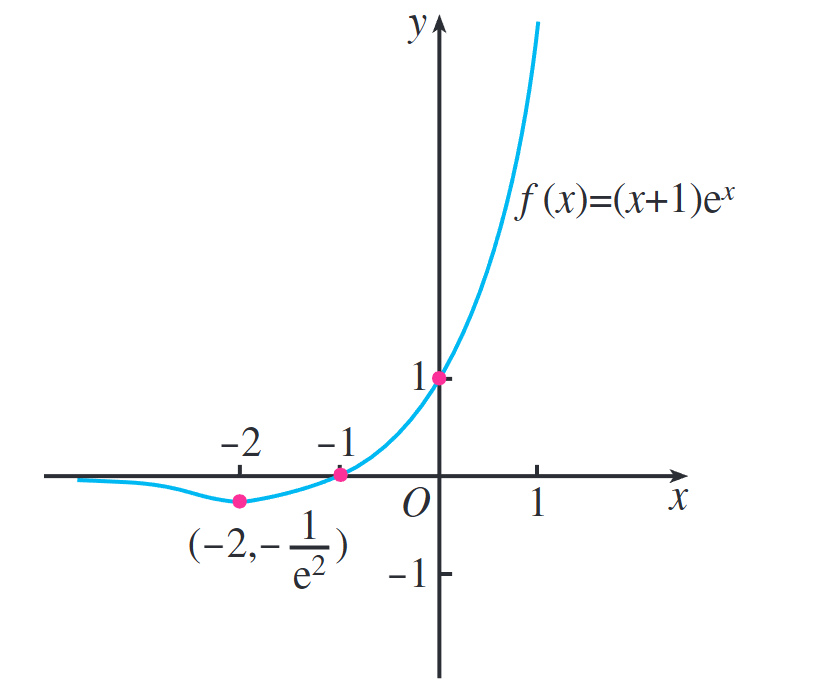
\includegraphics[width=0.5\textwidth]{绘图.png}
  \label{fig:single_image}
\end{figure}

\fbox{
  \parbox{0.95\textwidth}{
    tips：以上的解答均完全选自课本，从中可以看出，在高中范围内解题是是可以使用趋近于（极限）这一有利的数学概念的
    （尽管课内的内部不包括这一部分），因此在书写解答过程中，并不需要对极限讳莫如深。
  }
}
\vspace{2\baselineskip}

\noindent \textbf{例一}\;\;作函数 \(y = \dfrac{\mathrm{e}^x(2x - 1)}{x - 1}\) 的大致图象。
\vspace{20\baselineskip}

\newpage

\section{题型专练}
\subsection{函数不等式放缩}
\subsubsection{命题解析:常用放缩不等式}
指对函数与直线：
\\
\[
\ e^x \geq x+1  \;\;\;\;\;\;\;\; \ \ln (x) \leq x-1
\]
\\
\[
\ e^x \leq ex  \;\;\;\;\;\;\;\;   \ \ln (x) \leq \frac{x}{e}
\]
\\

指对函数与曲线：
\\
\[
 \ \ln (x) \geq 1-\frac{1}{x}
\]
\\
\[
 \ \begin{cases}\ln (x) \geq \frac{2(x-1)}{x+1} & , x \geq 1 \\ \ln (x)<\frac{2(x-1)}{x+1} & , x<1\end{cases}
\]
\\
\[
 \ \begin{cases}\ln (x) \leq \frac{1}{2}\left(x-\frac{1}{x}\right) & , x \geq 1 \\ \ln (x) \geq \frac{1}{2}\left(x-\frac{1}{x}\right) & , x \leq 1\end{cases}
\]
\\

三角函数型：
\\
\[
 \ \sin (x) \leq x \leq \tan (x) \quad, 0 \leq x<\frac{\pi}{2}
\]
\\
\begin{figure}[h]
    \centering % 整体居中
    % 第一张图：占页面宽度的0.45，居中
    \begin{minipage}[t]{0.5\textwidth}
        \centering
        % 替换为你的第一张图片路径（支持png/jpg/pdf）
        \includegraphics[width=\textwidth]{放缩1.png}
        % 可选：添加子标题（不需要可删除）
        \caption*{图1：$e^x$ 与 $x+1$ 的关系}
    \end{minipage}
    \hspace{0.05\textwidth} % 两张图之间的间距
    % 第二张图：占页面宽度的0.45，居中
    \begin{minipage}[t]{0.25\textwidth}
        \centering
        % 替换为你的第二张图片路径
        \includegraphics[width=\textwidth]{放缩2.png}
        % 可选：添加子标题（不需要可删除）
        \caption*{图2：$\sin x$、$x$、$\tan x$ 的关系}
    \end{minipage}
\end{figure}
\newpage
\begin{center}
    \fbox{tips:指数找基友,对数单身狗}
\end{center}



\subsubsection{例题}

例一 (2023 天津) 当 $x>0$ 时,证明 $\left(\frac{1}{x}+\frac{1}{2}\right) \ln (x+1)>1$.
\vspace{10\baselineskip}

例二 (2019 天津理数) 设函数 $f(x)=e^x \cos (x)$ , $g(x)$ 为 $f(x)$ 的导函数,当 $x \in\left[\frac{\pi}{4}, \frac{\pi}{2}\right]$ 时,求证 $f(x)+g(x)\left(\frac{\pi}{2}-x\right) \geq0$.
\vspace{10\baselineskip}

例三 (2024 和平一模) 已知函数 $f(x)=x \ln (x)$ , $g(x)=x(1-e^{x-1})$ , 设 $g(x)$ 在 $x=1$ 处的切线方程为 $y=k(x)$ ,求证:当 $x \in(1,+\infty)$ 时, $g(x)<k(x)$.
\vspace{10\baselineskip}

例四 (2022 天津) 证明: $\frac{e^{2 x}}{x(x+1)}>e$ , $x>0$.
\vspace{6\baselineskip}

\newpage
例五 (2024 南开二模) 已知函数 $f(x)=\sin x$ , $g(x)=1-\frac{x^2}{2}$
\begin{enumerate}
\item[(I)] 求曲线 $y=f(x)$ 在 $x=0$ 处的切线方程;
\item[(II)] 证明:对 $\forall x \in[0,+\infty)$ , $f'(x) \geq g(x)$ 恒成立.
\end{enumerate}
\vspace{24\baselineskip}

例六 (2024 部分区二模) 已知函数 $f(x)=e^x-a x$ , $a \in \mathbb{R}$
\begin{enumerate}
\item[(I)] 若曲线 $y=f(x)$ 在 $x=1$ 处的切线的斜率为2,求 $a$ 的值;
\item[(II)] 当 $a=0$ 时,证明: $\forall x \in(0,1)$ , $f(2 x)<\frac{1+x}{1-x}$.
\end{enumerate}
\vspace{20\baselineskip}

\newpage
\subsection{恒成立、存在性及参数取值问题}
\subsubsection{命题解析}
在导数题目中,我们往往要对等式或不等式进行变形处理,这里有两个常用的原则:
1. 指数找基友,对数单身狗;
2. 能参变分离就参变分离.

但很多时候二者无法同时实现,则须根据具体题目选择合适的方法。不过很多时候,当函数表达式过于复杂的时候,以上两种都很难实现,此时直接按照题目所给形式求导,或许能“拨开云雾见青天”。

\subsubsection{例题}

例一 (2025 天津) 已知函数 $f(x)=a x-(\ln x)^2$
\begin{enumerate}
\item[(I)] $a=1$ 时,求 $f(x)$ 在点 $(1, f(1))$ 处的切线方程;
\item[(II)] $f(x)$ 有3个零点 $x_1$ , $x_2$ , $x_3$ ,且 $x_1<x_2<x_3$
\begin{enumerate}
\item[(i)] 求 $a$ 的取值范围;
\item[(ii)] 我们后续完成
\end{enumerate}
\end{enumerate}
\vspace{20\baselineskip}

例二(2023新高考一卷)已知函数 \(f(x) = a(e^x + a) - x\)。

\begin{enumerate}
    \item 讨论 \(f(x)\) 的单调性；
    \item 证明：当 \(a > 0\) 时，\(f(x) > 2\ln a + \frac{3}{2}\)。
\end{enumerate}
\vspace{20\baselineskip}

例三 (2023 部分区二模) 设函数 $f(x)=a^x$ , $g(x)=\log_a x$ 其中 $a>1$ ,设 $h(x)=\frac{x^a}{f(x)}(x>0)$
\begin{enumerate}
\item[(I)] 当 $a=2$ 时,求 $h(x)$ 的单调区间;
\item[(II)] 曲线 $y=h(x)$ 与直线 $y=1$ 有且仅有两个交点,求 $a$ 的取值范围.
\end{enumerate}
\vspace{20\baselineskip}

\newpage
\subsection{分类讨论问题}
\subsubsection{命题解析}
在此类题目中,对含参数的二次函数进行讨论是重点和难点,一般来说我们有以下技巧:
1. 通过韦达定理观察两根的分布;
2. 可以尝试寻找该抛物线经过的定点,进而明确函数的基本走势;
3. 分类应做到不重不漏,在需要讨论的二次函数较为复杂时,可以把特殊点单独拿出来讨论(例如退化情况,即二次项系数为0,或是与x轴无交点)。

\subsubsection{例题}

例一 (2022 和平一模) 设函数 $f(x)=\ln (x+1)+a(x^2-x)$
\begin{enumerate}
\item[(I)] 当 $a=1$ 时,求曲线 $y=f(x)$ 在点 $(1, f(1))$ 处的切线方程;
\item[(II)] 讨论函数 $f(x)$ 极值点的个数,并说明理由;
\item[(III)] 若 $\forall x>0$ , $f(x) \geq0$ 成立,求 $a$ 的取值范围.
\end{enumerate}
\vspace{20\baselineskip}

例二 (2024 河西三模) 已知函数 $f(x)=-2 a \ln x-\frac{2}{x}$ , $g(x)=a x-(2 a+1) \ln x-\frac{2}{x}$ ,其中 $a \in \mathbb{R}$
\begin{enumerate}
\item[(I)] 若 $f'(2)=0$ ,求实数 $a$ 的值;
\item[(II)] 当 $a>0$ 时,求函数 $g(x)$ 的单调区间;
\item[(III)] 若存在 $x \in\left[\frac{1}{e}, e^2\right]$ ,使不等式 $f(x) \leq g(x)$ 成立,求 $a$ 的取值范围.
\end{enumerate}
\vspace{20\baselineskip}

例三 (2023 河东二模) 已知函数 $f(x)=x(\ln x-m-1)$ , $m \in \mathbb{R}$
\begin{enumerate}
\item[(I)] 若 $m=2$ ,求曲线 $y=f(x)$ 在点 $(e, f(e))$ 处的切线方程;
\item[(II)] 当 $x>1$ 时,求函数 $f(x)$ 的单调区间和极值;
\item[(III)] 若对于任意 $x \in[e, e^2]$ ,都有 $f(x)<4 \ln x$ 成立,求实数 $m$ 的取值范围.
\end{enumerate}
\vspace{20\baselineskip}

\newpage
\subsection{隐零点问题}
\subsubsection{命题解析}

我们经常利用零点存在定理来判断一个函数、导函数零点的存在性,但求出这个零点的具体数值往往并不容易,甚至是无法求解,这种必定存在但我们无法确定其值的零点就称为隐零点,在做题过程中,我们把它设为一个“未知数”,进而处理。

但是,我们可以通过以下方法挖掘这个零点的潜在信息,来解决问题:
1. 在可能出现零点的附近试数来卡出零点的大概范围;
2. 一个隐零点会对应一个方程,有些时候需要对这个方程进行处理来得到更多信息;有些时候需要利用这个等式将目标式进行变形(特别是用幂函数替换掉指对函数)。

值得注意的是,这种思想的运用是普遍的,也就是说,关键在于“隐”这种设而不求的思想而非“零点”,或许,我们还会遇到“隐极值点”的问题。

\subsubsection{例题}

例一  \;求函数 $f(x)=\ln (x)-x e^x+x$ 的最大值.
\vspace{13\baselineskip}

例二 (2018 天津理数) 设函数 $f(x)=a^x$ , $g(x)=\log_a x$ ,其中 $a>1$
\begin{enumerate}
\item[(I)] 求函数 $h(x)=f(x)-x \ln a$ 的单调区间;
\item[(II)] 若曲线 $y=f(x)$ 在点 $(x_1, f(x_1))$ 处的切线与曲线 $y=g(x)$ 在点 $(x_2, g(x_2))$ 处的切线平行,证明 $x_1+g(x_2)=-\frac{2 \ln \ln a}{\ln a}$;
\item[(III)] 证明当 $a \geq e^{\frac{1}{e}}$ 时,存在直线 $l$ ,使得 $l$ 是曲线 $y=f(x)$ 的切线,也是曲线 $y=g(x)$ 的切线.
\end{enumerate}
\vspace{24\baselineskip}

例三 (2023 河北一模) 已知函数 $f(x)=x-\ln x-2$
\begin{enumerate}
\item[(I)] 求曲线 $y=f(x)$ 在点 $(1, f(1))$ 处的切线方程;
\item[(II)] 讨论函数 $f(x)$ 的单调性;
\item[(III)] 若对任意的 $x \in(1,+\infty)$ ,都有 $x \ln x+x>k(x-1)$ 成立,求整数 $k$ 的最大值.
\end{enumerate}
\vspace{20\baselineskip}

例四 (2024 南开中学四月考) 已知函数 $f(x)=a e^x-\sin x-a$ ($e=2.718281\cdots$ 是自然对数的底数)
\begin{enumerate}
\item[(I)] 当 $a=3$ 时,求曲线 $y=f(x)$ 在点 $(0, f(0))$ 处的切线方程;
\item[(II)] 当 $a>0$ 时,函数 $f(x)$ 在区间 $\left(0, \frac{\pi}{2}\right)$ 内有唯一的极值点 $x_1$
\begin{enumerate}
\item[(i)] 求实数 $a$ 的取值范围;
\item[(ii)] 求证: $f(x)$ 在区间 $(0, \pi)$ 内有唯一的零点 $x_0$ ,且 $x_0<2 x_1$.
\end{enumerate}
\end{enumerate}
\vspace{20\baselineskip}


\newpage
\subsection{极值点偏移}
\subsubsection{命题解析}
对于二次函数,其函数值相等的两点的中点恰好是其极值点,这是由于二次函数的对称性造成的。对于更复杂的函数而言,其极值点两端的增长速度不同,这就造成了函数值相等两点的中点与极值点产生了不等式关系,我们称之为“偏移”。

需要注意的是,此种题型的上位概念是构造函数以比较某些特殊的取值的大小,尽管极值点偏移不可能出现在未来的高考试题中,但这种构造函数的思想却成为了考察的重点。

\begin{center}
% 外层figure环境（可选，也可只用center）
\begin{figure}[htbp]
    \centering
    % 子图(a)：lnx相关图像
    \subfloat[]{
        \begin{minipage}{0.48\textwidth}
            \centering
            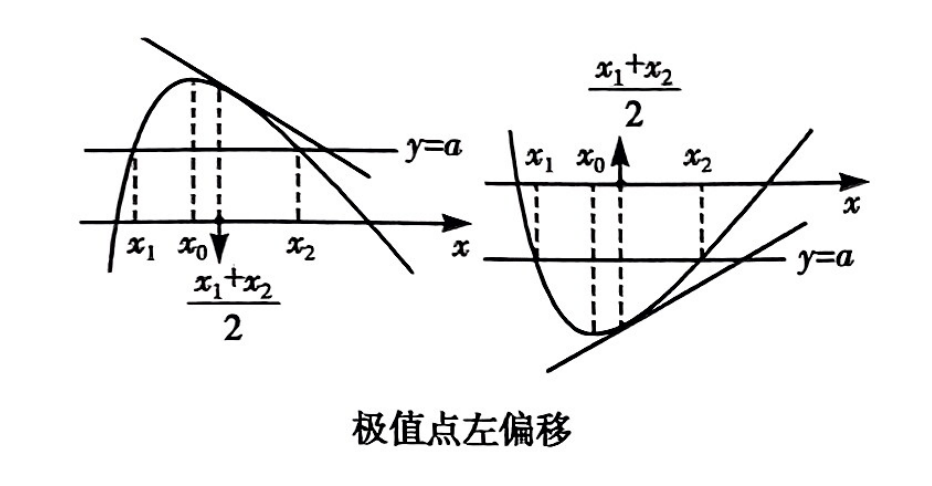
\includegraphics[width=0.95\textwidth]{image1.png}
        \end{minipage}
    }
    \hfill
    % 子图(b)：三角函数放缩图像
    \subfloat[]{
        \begin{minipage}{0.48\textwidth}
            \centering
            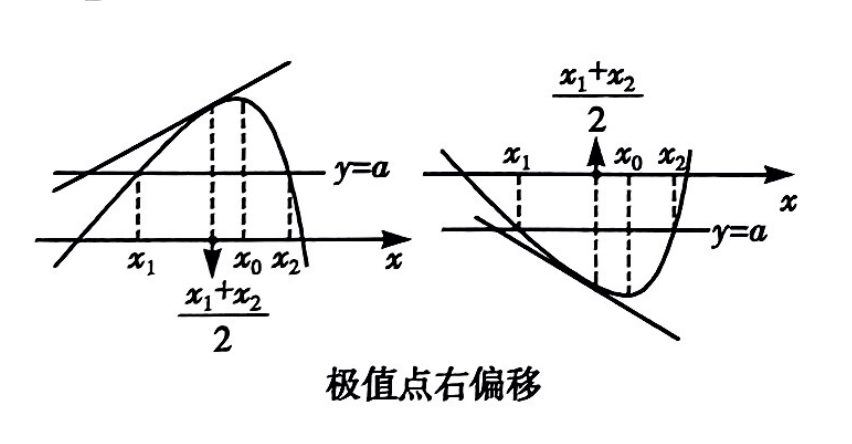
\includegraphics[width=0.95\textwidth]{image2.png}
        \end{minipage}
    }
    
    % 统一图例（包含子图说明）
    \caption{极值点偏移示意图}
    \label{fig:func_ineq_all}
\end{figure}
\end{center}

\begin{enumerate}
    \item 极值点左偏移的核心特征：$x_1 + x_2 > 2x_0$（其中 $x_0$ 为函数极值点），且在 $x = \frac{x_1 + x_2}{2}$ 处的切线与 $x$ 轴不平行。

具体性质:
\begin{enumerate}
    \item 若函数 $f(x)$ 的图象上凸（即 $f'(x)$ 单调递减），则满足：
    \[
    f'\left(\frac{x_1 + x_2}{2}\right) < f'(x_0) = 0;
    \]
    \item 若函数 $f(x)$ 的图象下凸（即 $f'(x)$ 单调递增），则满足：
    \[
    f'\left(\frac{x_1 + x_2}{2}\right) > f'(x_0) = 0.
    \]
\end{enumerate}

   \item  极值点右偏移的核心特征：$x_1 + x_2 < 2x_0$（其中 $x_0$ 为函数极值点），且在 $x = \frac{x_1 + x_2}{2}$ 处的切线与 $x$ 轴不平行。

具体性质：
\begin{enumerate}
    \item 若函数 $f(x)$ 的图象上凸（即 $f'(x)$ 单调递减），则满足：
    \[
    f'\left(\frac{x_1 + x_2}{2}\right) > f'(x_0) = 0;
    \]
    \item 若函数 $f(x)$ 的图象下凸（即 $f'(x)$ 单调递增），则满足：
    \[
    f'\left(\frac{x_1 + x_2}{2}\right) < f'(x_0) = 0.
    \]
\end{enumerate}
\end{enumerate}
\newpage
\subsubsection{例题}

例一 (2010 天津) 已知函数 $f(x)=x e^{-x}(x \in \mathbb{R})$
\begin{enumerate}
\item[(1)] 求函数 $f(x)$ 的单调区间和极值;
\item[(2)] 已知函数 $y=g(x)$ 的图象与函数 $y=f(x)$ 的图象关于直线 $x=1$ 对称,证明:当 $x>1$ 时, $f(x)>g(x)$;
\item[(3)] 如果 $x_1 \neq x_2$ ,且 $f(x_1)=f(x_2)$ ,求证: $x_1+x_2>2$.
\end{enumerate}
\vspace{20\baselineskip}

例二 (2022 河西期末) 已知函数 $f(x)=\ln x-a x(a \in \mathbb{R})$,e 为自然对数的底数
\begin{enumerate}
\item[(1)] 当 $a=\frac{1}{2}$ 时,求 $f(x)$ 的极值;
\item[(2)] 设函数 $g(x)=f(x)-2 x+1$ ,若 $g(x) \leq0$ 在其定义域内恒成立,求实数 $a$ 的最小值;
\item[(3)] 若关于 $x$ 的方程 $f(x)=x^2$ 恰有两个相异的实根 $x_1$ , $x_2$ ,求实数 $a$ 的取值范围,并证明 $x_1 x_2>1$.
\end{enumerate}
\vspace{20\baselineskip}

\newpage
\subsection{必要性探路(端点效应)}
\subsubsection{命题解析}

当题目涉及到一个含参数的恒成立问题,让我们求解参数的取值范围时,由于题目所给条件是恒成立,因此我们带入定义域中任一数值后均可得到一个关于参数的不等式,进而获得有关参数的取值范围,但由于我们只能取有限的点带入验证,因此我们得到的区间必然包括最终的答案,也就是说我们可以通过这种手段得到原题目的一个必要条件。

这样看来,这种方法看似不能帮助我们获得最终的答案,但很多时候,决定一个函数走势的,往往只是一些特殊的点(例如端点)以及该函数在此点的走势(导函数)。

\subsubsection{例题}


例一 (2022 全国乙卷) 已知函数 $f(x)=\ln (1+x)+a x e^{-x}$
\begin{enumerate}
\item[(1)] 当 $a=1$ 时,求曲线 $y=f(x)$ 在点 $(0, f(0))$ 处的切线方程;
\item[(2)] 若 $f(x)$ 在区间 $(-1,0)$,$(0,+\infty)$ 各恰有一个零点,求 $a$ 的取值范围.
\end{enumerate}
\vspace{20\baselineskip}

例二 (2023 天津一中一月考) 设函数 $f(x)=2 a x^2-2 a-\ln x$ , $g(x)=\frac{1}{x}-\frac{e}{e^x}$ ,其中 $a \in \mathbb{R}$ , e 为自然对数的底数
\begin{enumerate}
\item[(I)] 讨论 $f(x)$ 的单调性;
\item[(II)] 证明:当 $x>1$ 时, $g(x)>0$;
\item[(III)] 若不等式 $f(x)>g(x)$ 在 $x \in(1,+\infty)$ 时恒成立,求 $a$ 的取值范围.
\end{enumerate}
\vspace{20\baselineskip}

\newpage
\subsection{导数数列联袂不等式}
\subsubsection{命题解析}
在此题型中需要利用导数的知识得到恰当的不等式(一般来说,前问会给出一定的提示),再巧妙地用 $n$ 替换函数不等式中的量,进而利用这个不等式进行证明。

在本题中,有一些常见的技巧:
1. 累乘法和累加法--通过恰当变形来达到消项化简;
2. 数列求和及放缩技巧(例如错位相减、裂项相消和丢项放缩);
3. 对目标不等式进行处理--例如对于连乘式,我们可以通过取对数的方法处理(加法总是比乘法简单的);
4. 化整为零--通过数列中每一项的放缩来得到最终放缩;
5. 大 $n$ 验放缩,小 $n$ 调细节--无论是在数列放缩还是在导数放缩中,当自变量较大的时候,放缩就容易出现问题,具体表现为放缩式与目标函数的差距过大,放缩效果难以保证,因此需要保证当自变量趋近于无穷时,两式为同阶函数。如果我们进行了恰当的放缩避免了上述情况,那么 $n$ 较小时的误差就成为了主要误差,基于这种情况,对于一些严格的不等式,我们可以对前几项采取照抄不放缩的方法,这样就可以让我们的放缩更为精确。

\subsubsection{例题}

例一 (2023 和平一模) 设函数 $f(x)=e^x-a x$ , $g(x)=\ln (x+2)-a$
\begin{enumerate}
\item[(1)] 证明: $f'(x)>g(x)$ 恒成立;
\item[(2)] 证明: $\ln 2+\left(\ln \frac{3}{2}\right)^2+\left(\ln \frac{4}{3}\right)^3+\cdots+\left(\ln \frac{n+1}{n}\right)^n<\frac{e}{e-1}, n \in \mathbb{N}^*$.
\end{enumerate}
\vspace{20\baselineskip}

例二 (2023 天津) 已知函数 $f(x)=\left(\frac{1}{x}+\frac{1}{2}\right) \ln (x+1)$
\begin{enumerate}
\item[(1)] 求曲线 $y=f(x)$ 在 $x=2$ 处切线的斜率;
\item[(2)] 当 $x>0$ 时,证明: $f(x)>1$;
\item[(3)] 证明: $\frac{5}{6}<\ln (n!)-\left(n+\frac{1}{2}\right) \ln n+n \leq1, n \in \mathbb{N}^*$.
\end{enumerate}
\vspace{20\baselineskip}

\newpage
\subsection{双变量不等式}
\subsubsection{命题解析}
导数题目中通常的不等式是建立在单个变量上的,当变量推至两个甚至多个,其证明的难度也随着上升。此题型是近年高考绝对热点和难点,这个板块的技巧浩如烟海,难度更是达到了整个高中数学的顶峰,这里我们只介绍一种最简单的小分类--比值换元法。

我们都知道:双变量难以处理而单变量较为容易,因此我们可以通过一些手段将多变量转化为单变量,其中重要手段之一就是比值换元,即通过等式的变形,来达到题目中出现的两个变量均以比值的形式出现,这样就可以用单变量替换多变量。

\subsubsection{例题}

例零\; 证明下述不等式(对数均值不等式)
\[
\sqrt{a b}<\frac{a-b}{\ln a-\ln b}<\frac{a+b}{2}
\]
其中 $a>0$ , $b>0$ , $a \neq b$.
\vspace{10\baselineskip}


例一 (2020 天津) 已知函数 $f(x)=x^3+k \ln x(k \in \mathbb{R})$ , $f'(x)$ 为 $f(x)$ 的导函数
\begin{enumerate}
\item[(I)] 当 $k=6$ 时,
\begin{enumerate}
\item[(i)] 求曲线 $y=f(x)$ 在点 $(1, f(1))$ 处的切线方程;
\item[(ii)] 求函数 $g(x)=f(x)-f'(x)+\frac{9}{x}$ 的单调区间和极值;
\end{enumerate}
\item[(II)] 当 $k \geq-3$ 时,求证:对任意的 $x_1,x_2 \in[1,+\infty)$ ,且 $x_1>x_2$ ,有:
\[
\frac{f'\left(x_1\right)+f'\left(x_2\right)}{2}>\frac{f\left(x_1\right)-f\left(x_2\right)}{x_1-x_2}
\]
\end{enumerate}
\vspace{22\baselineskip}

例二(2022南开期末)已知函数 \(f(x) = 2\ln x - ax\)，\(a \in \mathbb{R}\)。

\begin{enumerate}
    \item[(1)] 当 \(a = 3\) 时，求函数 \(f(x)\) 的单调区间；
    \item[(2)] 若关于 \(x\) 的不等式 \(f(x) \leq ax^2 + (a-2)x - 2\) 恒成立，求整数 \(a\) 的最小值；
    \item[(3)] 是否存在一条直线与函数 \(y = f(x) + \frac{1}{2}x^2\) 的图象相切于两个不同的点？并说明理由。
\end{enumerate}
\vspace{25\baselineskip}
\newpage 

\subsection{同构问题}
\subsubsection{命题解析}
在导数题目中,我们经常会遇到一些看似复杂的函数,但通过一些变形处理后,就会发现它们与我们熟悉的函数具有相同的单调性、极值点分布等性质,这就是所谓的同构问题。在处理同构问题时,我们需要注意以下几点:
1. 通过适当的变形来揭示函数的本质特征,例如通过对数、指数等操作来简化函数的表达式;
2. 识别函数的基本类型,例如幂函数、指数函数、对数函数等,并利用这些类型的已知性质来分析函数的行为;
3. 在分析函数的单调性、极值点等性质时,要注意函数的定义域和可能的特殊点,以确保分析的准确性.

确切的说，同构就是一个把等式两边变为$f(u(x))=f(v(x))$的过程，这样，当$f(x)$性质较好时，我们可以在某种意义下脱去函数外衣，直接研究$u(x)$和$v(x)$的关系。

下面是几个常见的同构方法：
\begin{enumerate}
    \item 积型: \(ae^a \leq b\ln b\)

    同左侧结构:
    \[
    ae^a \leq b\ln b \implies a \cdot e^a \leq \ln b \cdot e^{\ln b} \Rightarrow f(x) = xe^x.
    \]

    同右侧结构:
    \[
    ae^a \leq b\ln b \implies e^a \cdot \ln e^a \leq b \cdot \ln b \Rightarrow f(x) = x\ln x.
    \]

    两侧取对数:
    \[
    ae^a \leq b\ln b \implies a + \ln a \leq \ln b + \ln(\ln b) \Rightarrow f(x) = x + \ln x.
    \]
    （取对数最为便捷，且单调性易知）

    \item 商型: \(\dfrac{e^a}{a} < \dfrac{b}{\ln b}\)

    同左侧结构:
    \[
    \frac{e^a}{a} < \frac{b}{\ln b} \implies \frac{e^a}{a} < \frac{e^{\ln b}}{\ln b} \Rightarrow f(x) = \frac{e^x}{x}.
    \]

    同右侧结构:
    \[
    \frac{e^a}{a} < \frac{b}{\ln b} \implies \frac{e^a}{\ln e^a} < \frac{b}{\ln b} \Rightarrow f(x) = \frac{x}{\ln x}.
    \]

    两侧取对数:
    \[
    \frac{e^a}{a} < \frac{b}{\ln b} \implies a - \ln a < \ln b - \ln(\ln b) \Rightarrow f(x) = x - \ln x.
    \]

    \item 和差型: \(e^a \pm a > b \pm \ln b\)

    同左侧结构:
    \[
    e^a \pm a > b \pm \ln b \implies e^a \pm a > e^{\ln b} \pm \ln b \Rightarrow f(x) = e^x \pm x.
    \]

    同右侧结构:
    \[
    e^a \pm a > b \pm \ln b \implies e^a \pm \ln e^a > b \pm \ln b \Rightarrow f(x) = x \pm \ln x.
    \]

    \item 若式子无法直接进行变形同构，往往需要凑常数、凑参数或凑变量，如两边同乘以 \(x\)，同加上 \(x\) 等，再用上述方式变形。常见的有:
    \[
    ae^{ax} > \ln x \implies axe^{ax} > x\ln x;\ a^x > \log_a x \implies e^{x\ln a} > \frac{\ln x}{\ln a} \implies (x\ln a)e^{x\ln a} > x\ln x
    \]

\end{enumerate}

\subsubsection{例题}

例一\;\; \noindent 若不等式 \(mx e^{mx^2} \geq \ln x\) 恒成立，求 \(m\) 的取值范围。
\vspace{10\baselineskip}

例二 \;\;已知函数 \(f(x) = (x-1)e^x - ax\)（\(a \in \mathbb{R}\) 且 \(a\) 为常数）。

\begin{enumerate}
    \item 讨论 \(f(x)\) 的极值点个数；
    \item 若 \(f(x) \geq \ln x - e^x + 1\) 对任意的 \(x \in (0,+\infty)\) 恒成立，求实数 \(a\) 的取值范围。
\end{enumerate}
\newpage
\section{综合练习}

\noindent 1. （2022新高考一卷）已知正四棱锥的侧棱长为 \(l\)，其各项顶点都在同一球面上，若该球的体积为 \(36\pi\)，且 \(3 \le l \le 3\sqrt{3}\)，则该正四棱锥体积的取值范围是(\;\;\;)

\begin{enumerate}[label=\Alph*., noitemsep]
    \item \(\left[18, \dfrac{81}{4}\right]\)
    \item \(\left[\dfrac{27}{4}, \dfrac{81}{4}\right]\)
    \item \(\left[\dfrac{27}{4}, \dfrac{64}{3}\right]\)
    \item \(\left[18, 27\right]\)
\end{enumerate}
\vspace{3\baselineskip}

\noindent 2.（2022新高考一卷）设 \(a = 0.1e^{0.1}\)，\(b = \dfrac{1}{9}\)，\(c = -\ln 0.9\)，则(\;\;\;)

\begin{enumerate}[label=\Alph*., noitemsep]
    \item \(a < b < c\)
    \item \(c < b < a\)
    \item \(c < a < b\)
    \item \(a < c < b\)
\end{enumerate}
\vspace{5\baselineskip}

\noindent 3.（2025天津） 已知函数 \(f(x) = ax - (\ln x)^2\)

\begin{enumerate}
    \item[(I)] 当 \(a=1\) 时，求 \(f(x)\) 在点 \((1, f(1))\) 处的切线方程；
    \item[(II)] \(f(x)\) 有 3 个零点 \(x_1, x_2, x_3\)，且 \(x_1 < x_2 < x_3\)。
    \begin{enumerate}
        \item[(i)] 求 \(a\) 的取值范围；
        \item[(ii)] 证明：\((\ln x_2 - \ln x_1) \cdot \ln x_3 < \dfrac{4e}{e-1}\)。
    \end{enumerate}
\end{enumerate}

\newpage
\noindent 4.（2018天津理数）设函数 \(f(x) = e^x \cos x\)，\(g(x)\) 为 \(f(x)\) 的导函数。

\begin{enumerate}
    \item[(1)] 求 \(f(x)\) 的单调区间；
    \item[(2)] 当 \(x \in \left[\frac{\pi}{4}, \frac{\pi}{2}\right]\) 时，证明：\(f(x) + g(x)\left(\frac{\pi}{2} - x\right) \geq 0\)；
    \item[(3)] 设 \(x_n\) 为函数 \(u(x) = f(x) - 1\) 在区间 \(\left(2n\pi + \frac{\pi}{4}, 2n\pi + \frac{\pi}{2}\right)\) 内的零点，其中 \(n \in \mathbb{N}\)，证明：
    \[
    2n\pi + \frac{\pi}{2} - x_n < \frac{e^{-2n\pi}}{\sin x_0 - \cos x_0}.
    \]
\end{enumerate}
\vspace{20\baselineskip}

\noindent 5. （2021南开期末）已知函数 \(f(x) = x\ln x - 1\)，\(g(x) = ax^2 - (a-2)x\)。

\begin{enumerate}
    \item[(1)] 求 \(f(x)\) 的最小值；
    \item[(2)] 设函数 \(h(x) = f'(x) - g(x)\)，讨论 \(h(x)\) 的单调性；
    \item[(3)] 设函数 \(G(x) = g(x) + (a-2)x\)，若函数 \(f(x)\) 的图像与 \(G(x)\) 的图像有 \(A(x_1, y_1)\)，\(B(x_2, y_2)\) 两个不同的交点，证明：\(\ln(x_1x_2) > 2 + \ln 2\)。
\end{enumerate}
\vspace{20\baselineskip}
\newpage

\noindent 6.（2022新高考二卷）已知函数 \(f(x) = x e^{ax} - e^x\).

\begin{enumerate}
    \item[(1)] 当 \(a = 1\) 时，讨论 \(f(x)\) 的单调性；
    \item[(2)] 当 \(x > 0\) 时，\(f(x) < -1\)，求 \(a\) 的取值范围；
    \item[(3)] 设 \(n \in \mathbb{N}^*\)，证明：
    \[
    \frac{1}{\sqrt{1^2+1}} + \frac{1}{\sqrt{2^2+2}} + \cdots + \frac{1}{\sqrt{n^2+n}} > \ln(n+1).
    \]
\end{enumerate}
\vspace{20\baselineskip}

\noindent 7.(2022南开期末)已知函数 \(f(x) = 2\ln x - ax\)，\(a \in \mathbb{R}\)。

\begin{enumerate}
    \item[(1)] 当 \(a = 3\) 时，求函数 \(f(x)\) 的单调区间；
    \item[(2)] 若关于 \(x\) 的不等式 \(f(x) \leq ax^2 + (a-2)x - 2\) 恒成立，求整数 \(a\) 的最小值；
    \item[(3)] 是否存在一条直线与函数 \(y = f(x) + \frac{1}{2}x^2\) 的图象相切于两个不同的点？并说明理由。
\end{enumerate}
\newpage

\noindent 8. (2022天津)已知 \(a,b \in \mathbb{R}\)，函数 \(f(x) = e^x - a\sin x\)，\(g(x) = b\sqrt{x}\)。

\begin{enumerate}
    \item[(I)] 求函数 \(y = f(x)\) 在 \((0, f(0))\) 处的切线方程；
    \item[(II)] 若 \(y = f(x)\) 和 \(y = g(x)\) 有公共点
    \begin{enumerate}
        \item[(i)] 当 \(a = 0\) 时，求 \(b\) 的取值范围；
        \item[(ii)] 求证：\(a^2 + b^2 > e\)。
    \end{enumerate}
\end{enumerate}
\vspace{25\baselineskip}



\noindent 9.(2024新高考一卷)已知函数 \(f(x) = \ln \dfrac{x}{2 - x} + ax + b(x - 1)^3\)。
\begin{enumerate}
    \item[(1)] 若 \(b = 0\)，且 \(f'(x) \ge 0\)，求 \(a\) 的最小值；
    \item[(2)] 证明：曲线 \(y = f(x)\) 是中心对称图形；
    \item[(3)] 若 \(f(x) > -2\) 当且仅当 \(1 < x < 2\)，求 \(b\) 的取值范围。
\end{enumerate}



\end{document}

